\section{Benchmarks}
\label{sec:benchmark}

In this section, we demonstrate the efficacy of our approaches via a set of benchmarks.

\subsection{MPI Paths Reconstruction}

In our experiment, we need to measure not only the performance of MPI routines but also loads on physical links and number of hops of path that MPI takes to move data from a set of sources to a set of destination. The load and hops informaiton can reveal insight of performance difference between MPI and our framework OPTIQ. Thus reconstructing MPI's paths is necessary to get load and hops information.

We reconstruct MPI's paths based on our understanding of default routing algorithms described in \cite{Chen:BGQ}. For each pair of source and destination, we start at a source node and follow the rules of the routing algorithm to move data from the source node to its destination. We then record paths for all the pairs and use them to calculate load and number of hops. 

\subsection{Communication Patterns}
In this paper we demostrate data movement performance of our OPTIQ framework and existing MPI's routines on the following communication patters:

\begin{figure}[!htb]
\vspace{-0.1in}
\centering
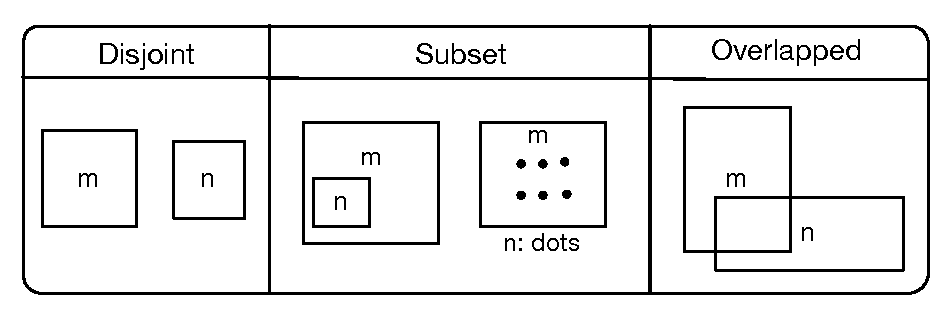
\includegraphics[scale=0.55]{figures/patterns.pdf}
\vspace{-0.1in}
\caption{Communication patterns}
\vspace{-0.1in}
\label{fig:patterns}
\end{figure}

\begin{itemize}
\item Subgroup Data Aggregation: a special case of All to many (or many to many.)
\item Many to many: disjoint sets.
\item Many to many: overlapped sets.
\item Many to many: subsets. In this category, there are 2 sub types: (Type 1) concetrated subset of destinations and (Type 2) distributed destination nodes as in I/O data aggregation.
\end{itemize}

We carried a set of experiments to study the system's behavior in various patterns and demontrate throughput improvement.

\subsection{Experimental results}

In the experiments, we collected the throughput and loading related information while varying communication patterns, partition sizes, message sizes, number of MPI ranks per node.
The results of 96 experiments in the Figure \ref{fig:96tests_512} show the throughput of 512-nodes partition with in 96 experiments of 3 above communication patterns.

\begin{figure}[!htb]
\vspace{-0.1in}
\centering
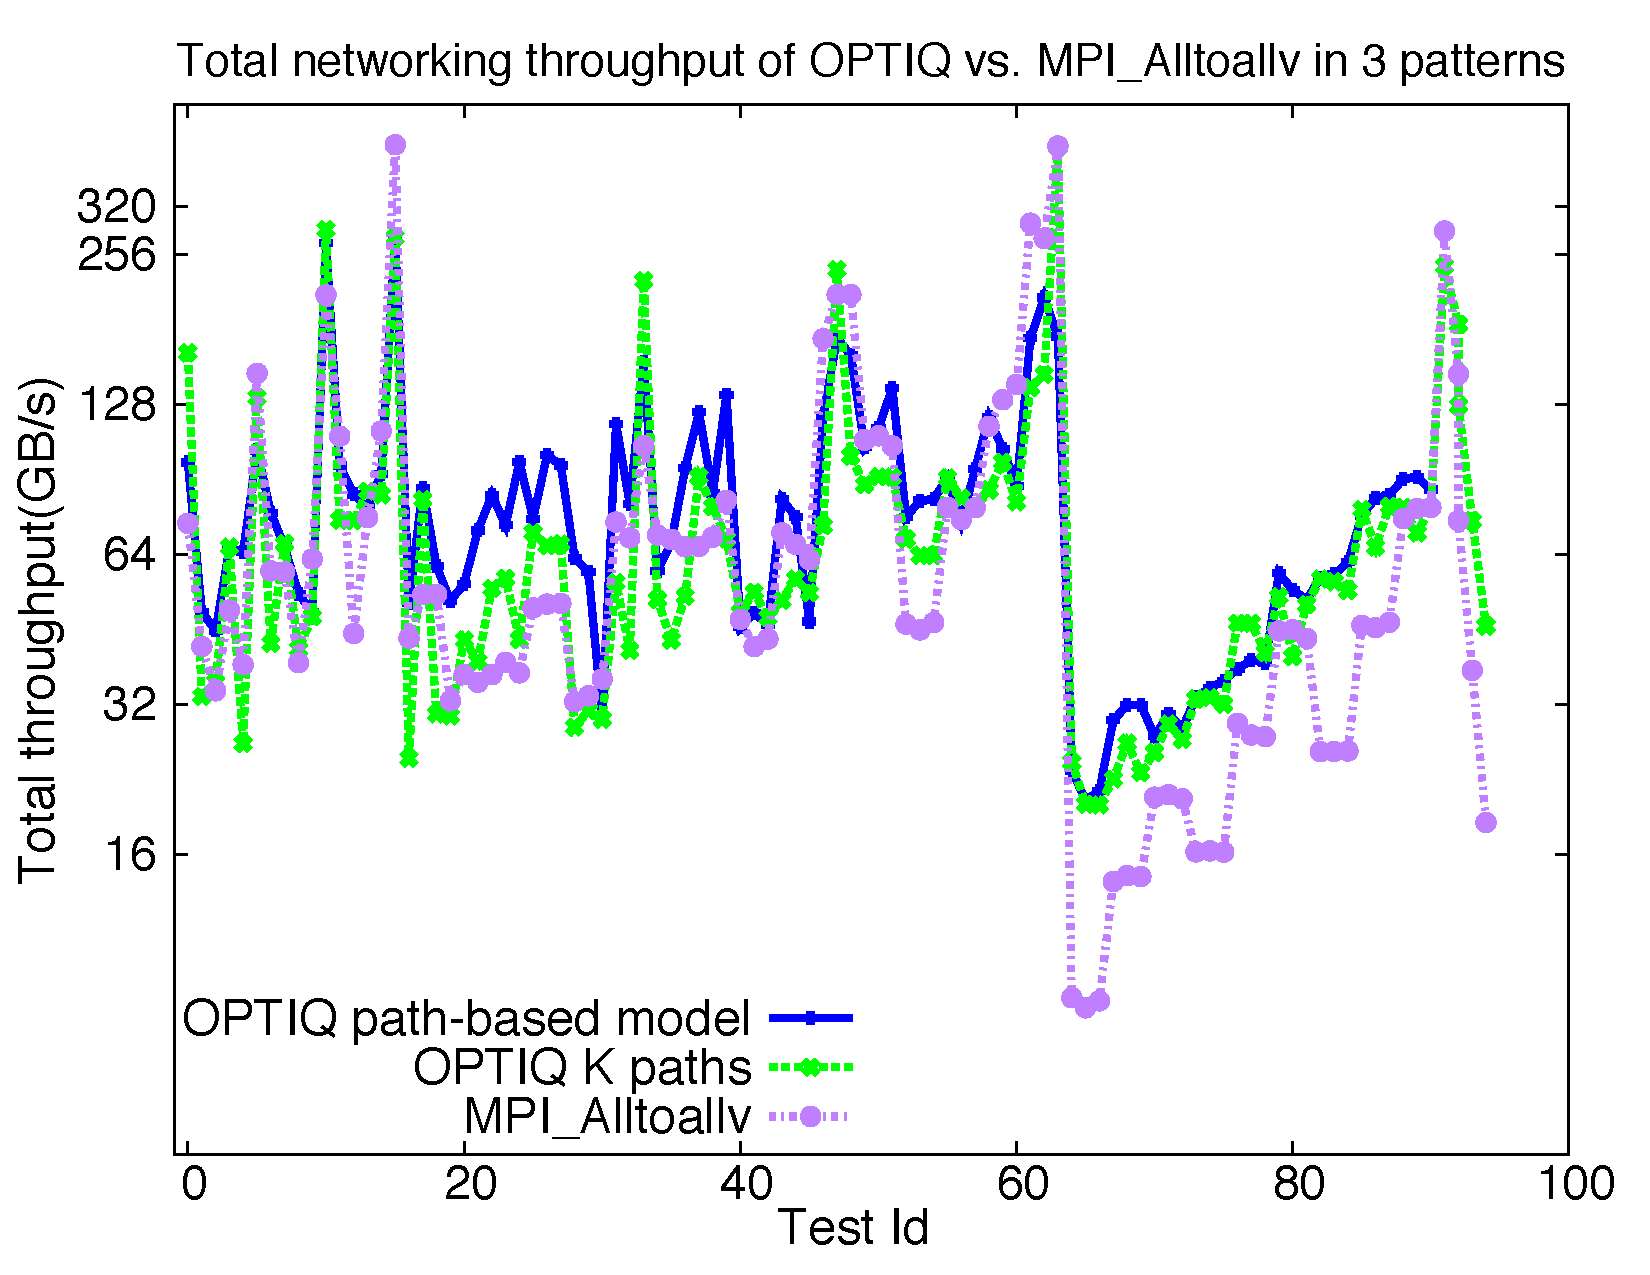
\includegraphics[scale=0.30]{figures/96tests_512.pdf}
\vspace{-0.1in}
\caption{Communication patterns}
\vspace{-0.1in}
\label{fig:96tests_512}
\end{figure}

The Table \ref{tbl:experiment} describes the details of the experiments.

\begin{table}[h]
\begin{center}
    \begin{tabular}{ | p{1cm} | l | p{5cm} |}
    \hline
    Pattern & Test Ids & Sets of source/destination \\ \hline
    Disjoint & 0-15 & Vary the size of sources and destinations sets from N/16 to N/2 \\ \hline
    Overlap & 16-63 & Vary the size of sources and destinations sets from N/16 to N/2, overlapped size varies from 1/8 to 1/2 of the source size \\ \hline
    Subset: Type 1 & 63-90 & Vary the size of source set from N/8 to N/2 and destination set from N/16 to N/4 lying inside source set \\ \hline
    Subset: Type 2 & 91-95 & Vary the subgroup size from 4, 8, 16, 32 to 64. The destination of each subgroup is in the middle of the group \\
    \hline
    \end{tabular}

    \caption{Experiments description}
    \label{tbl:experiment}

\end{center}
\end{table}

In the next subsections, we go into each communication and study in details the system's behaviors and performance.

\subsubsection{Disjoint sets of sources and destinations}

\begin{figure}[!htb]
\vspace{-0.1in}
\centering
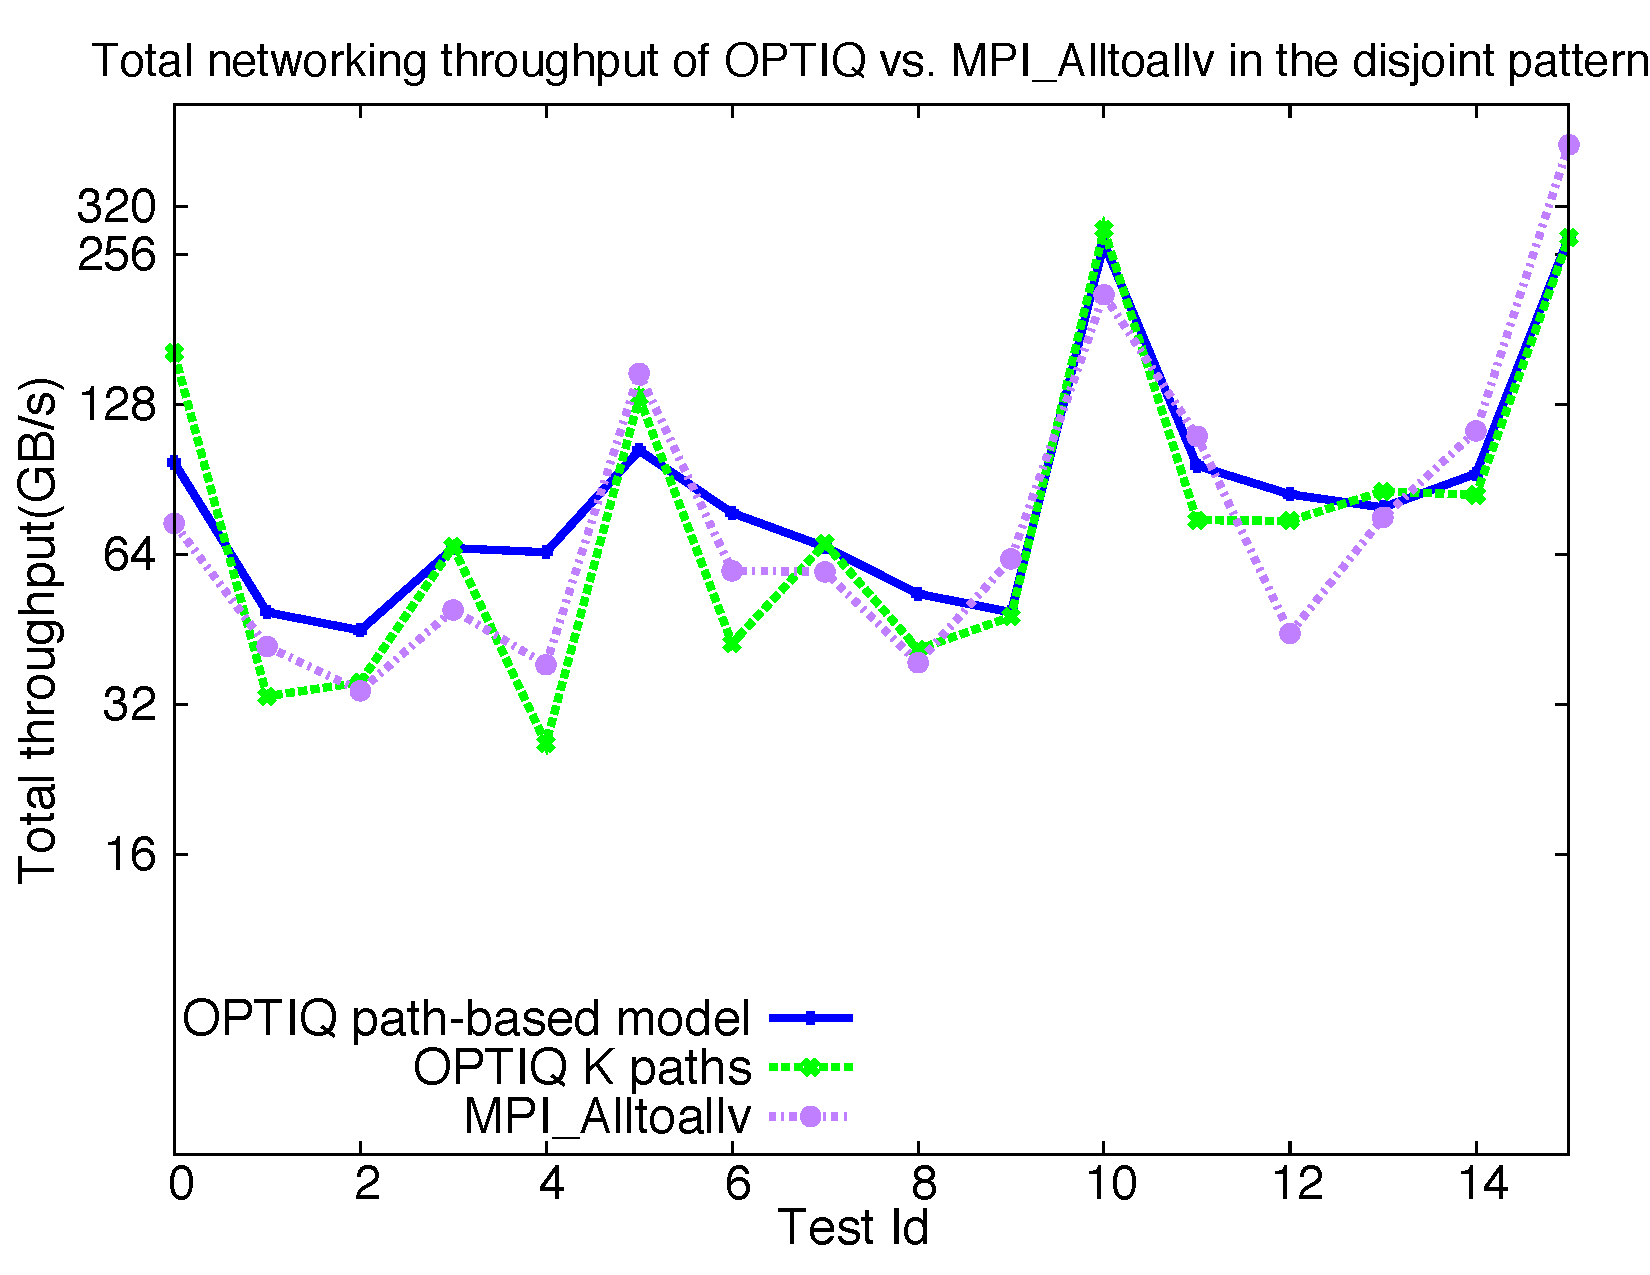
\includegraphics[scale=0.30]{figures/disjoint_512.pdf}
\vspace{-0.1in}
\caption{Disjoint sets - 512}
\vspace{-0.1in}
\label{fig:disjoint_512}
\end{figure}

\subsubsection{Overlaped sets of sources and destinations}

\begin{figure}[!htb]
\vspace{-0.1in}
\centering
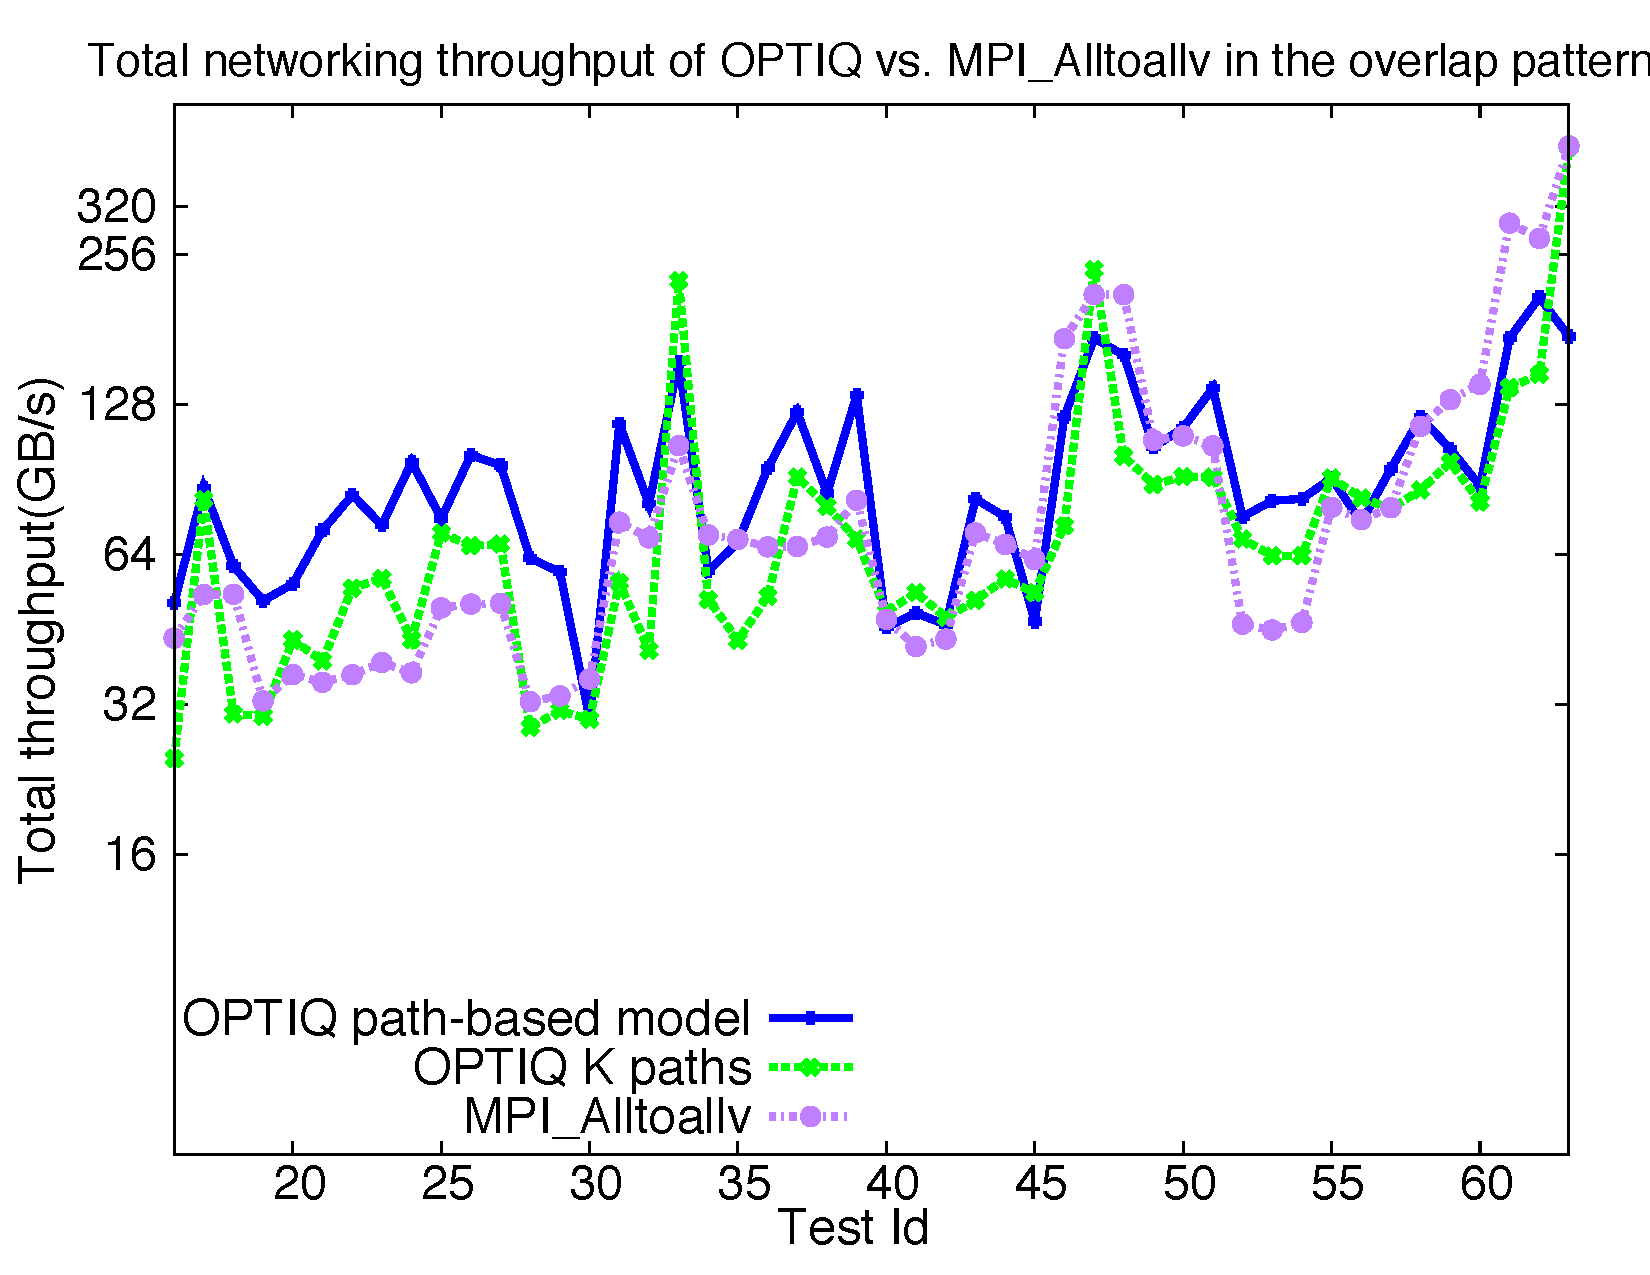
\includegraphics[scale=0.30]{figures/overlap_512.pdf}
\vspace{-0.1in}
\caption{Overlapped sets 512 nodes}
\vspace{-0.1in}
\label{fig:overlap_512}
\end{figure}

\subsubsection{Subset - Type 1}

\begin{figure}[!htb]
\vspace{-0.1in}
\centering
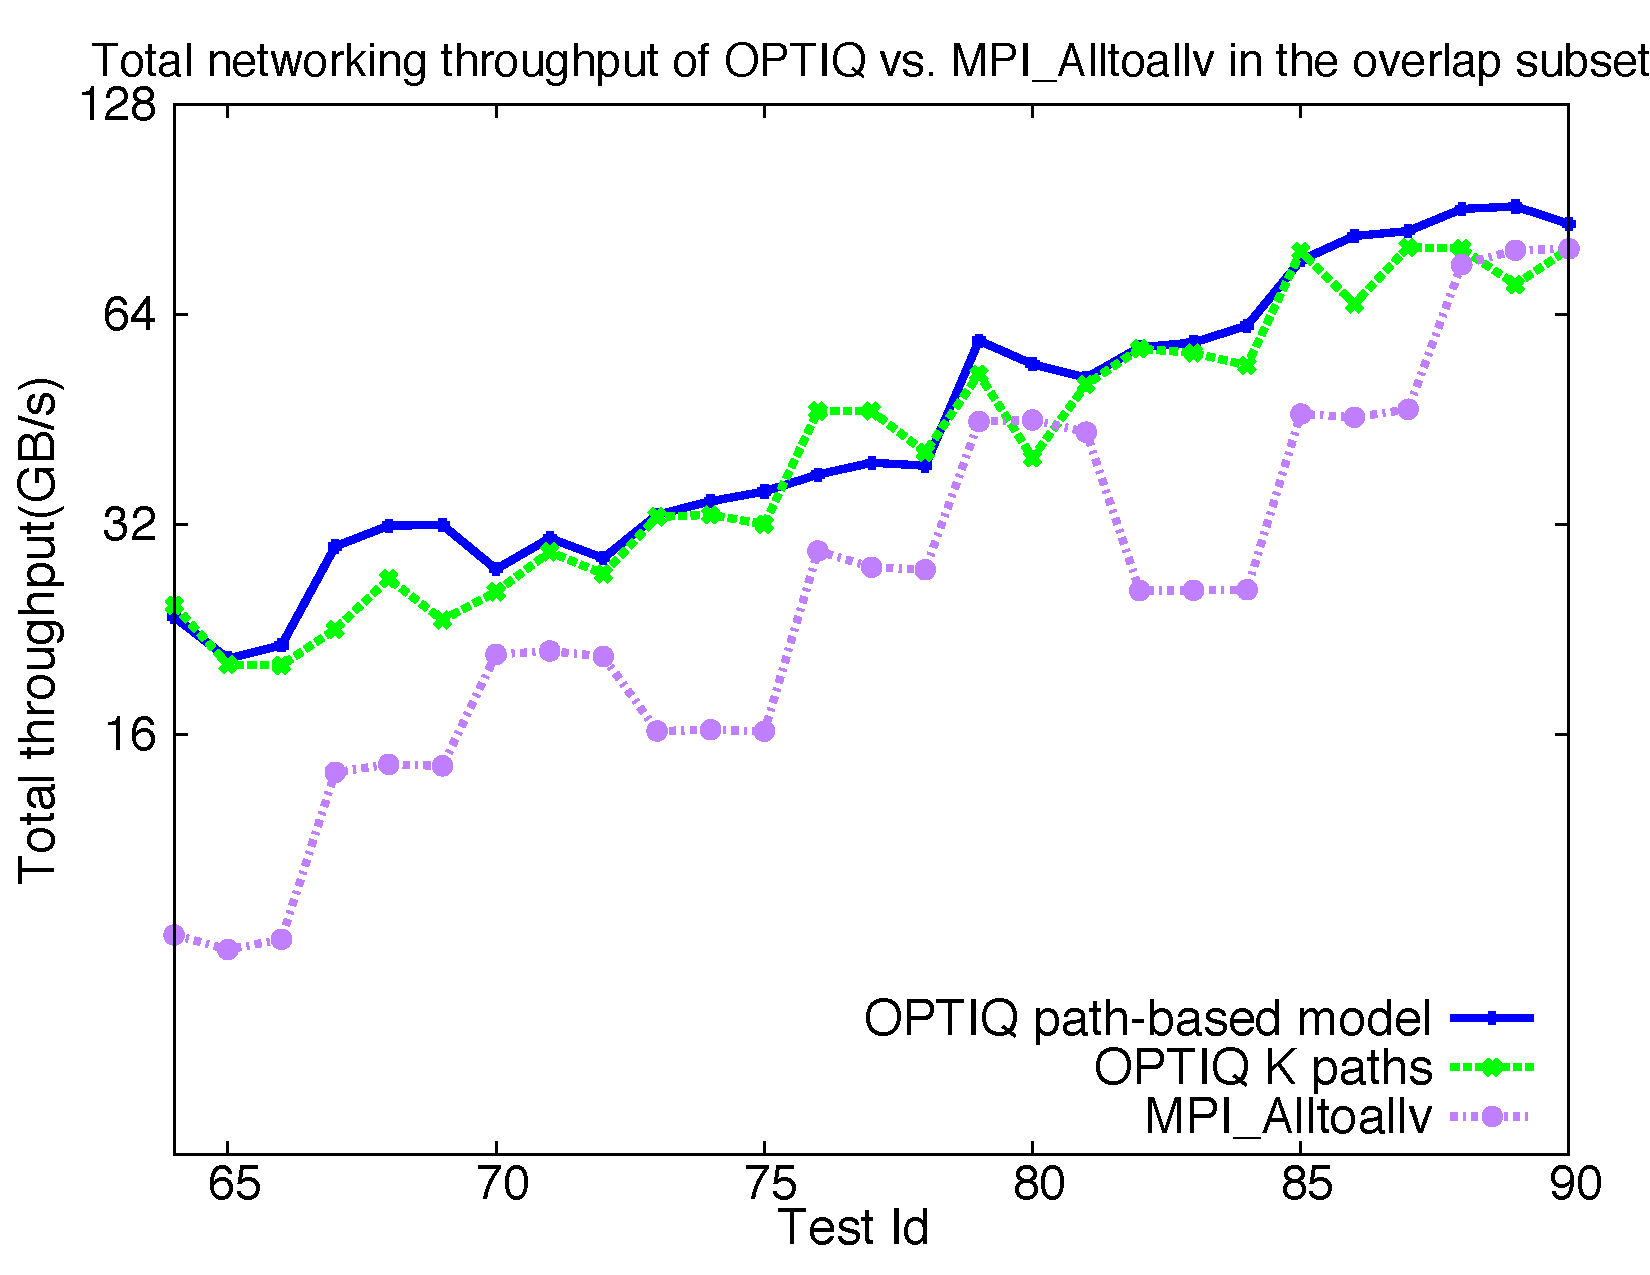
\includegraphics[scale=0.30]{figures/subset_512.pdf}
\vspace{-0.1in}
\caption{Subset 512 nodes}
\vspace{-0.1in}
\label{fig:subset_512}
\end{figure}

\subsubsection{Subgroup - Type 2 Data Aggregation}

In the subgroup data aggregation experiment, we aggregated data within a subgroup to one node in the subgroup. In this experiment, we used a 512-nodes partition. The partition was divided into subgroup of size 4, 8, 16, 32, and 64 nodes each. One node in the middle of a subgroup was selected as the destination to aggregate data from all nodes in the subgroup(including itself). The data size is 1MB. We aggregate data using MPI\_Alltoallv and our framework for 20 times, measured and reported the average of the measurements. The aggregation bandwidths are shown in Figure \ref{fig:aggbw}.

\begin{figure}[!htb]
\vspace{-0.1in}
\centering
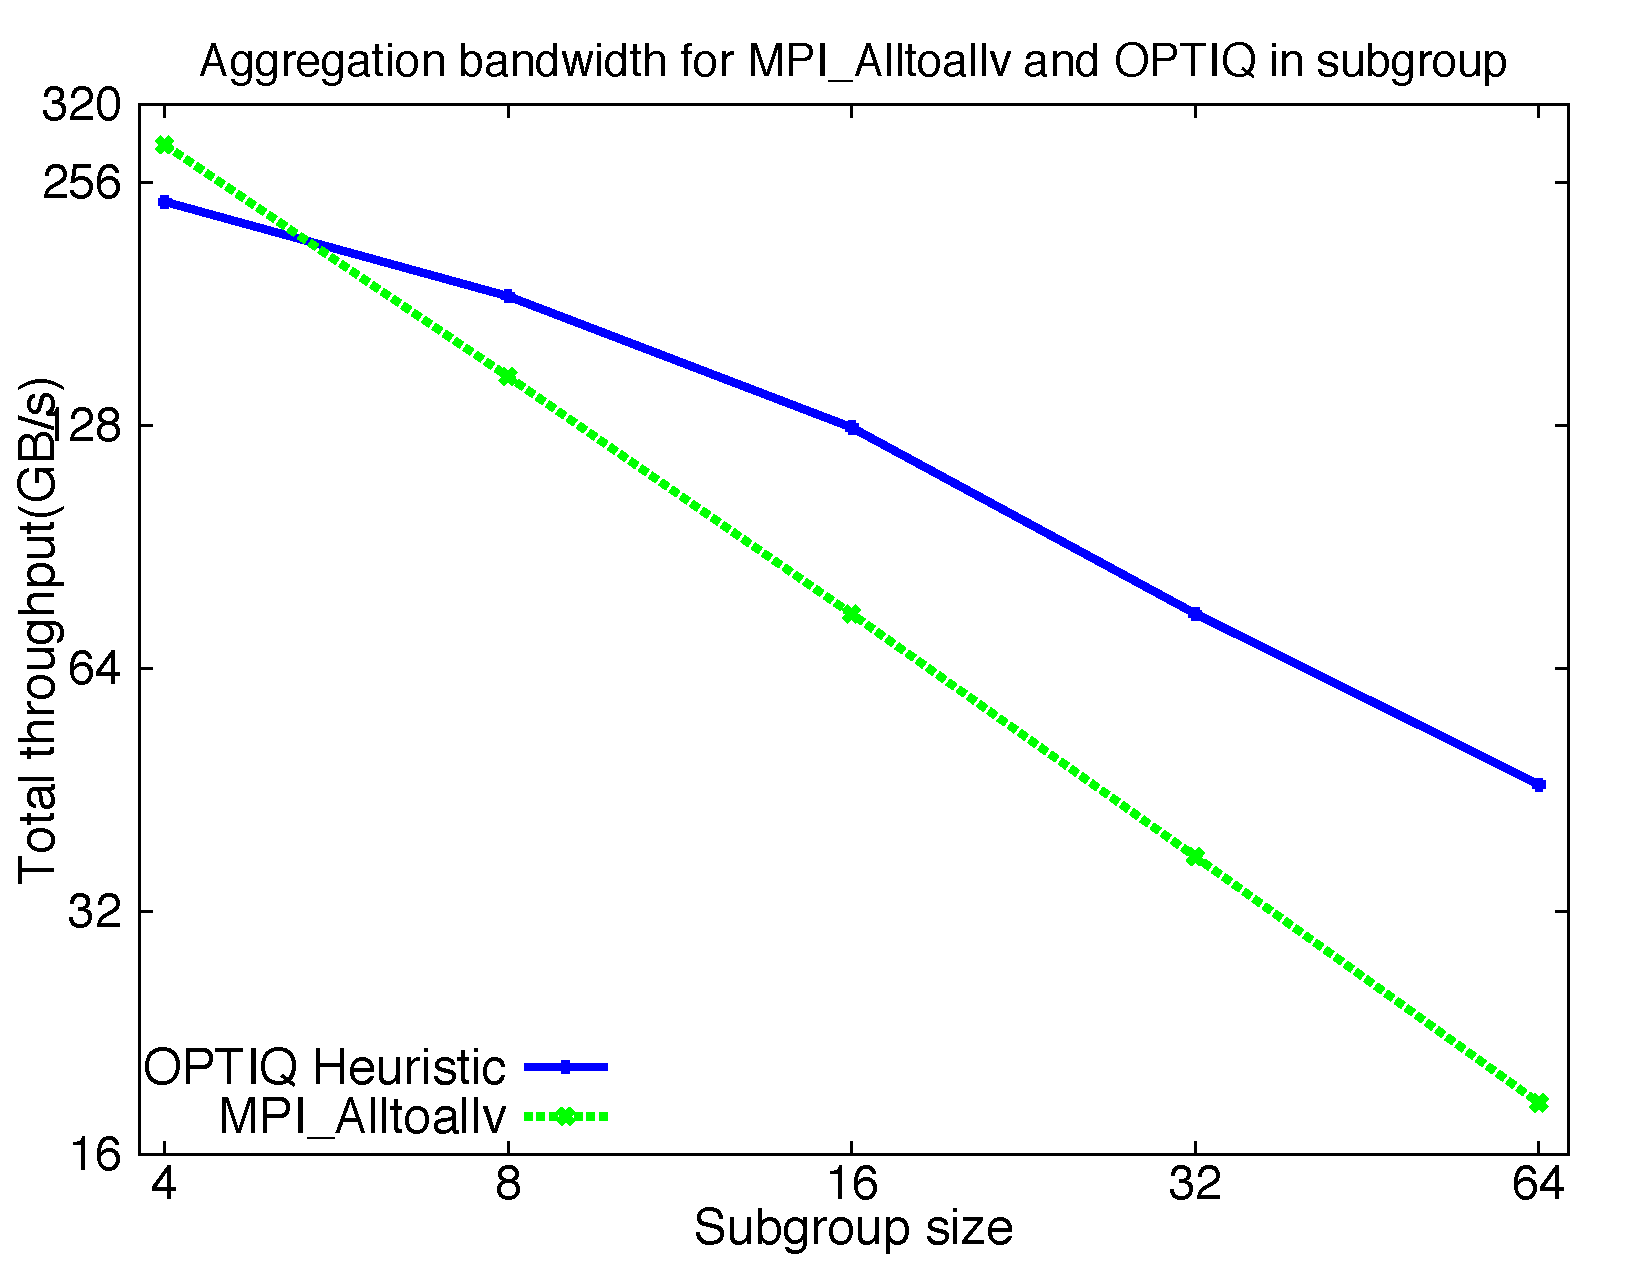
\includegraphics[scale=0.30]{figures/agg.pdf}
\vspace{-0.1in}
\caption{Aggregation bandwidth}
\vspace{-0.1in}
\label{fig:aggbw}
\end{figure}

As we can see in the figure, our work shows better performance as we increased subgroup size due to more balanced networking load. At the beginning when teh size of subgroups is 4, MPI\_Alltoallv performed better. But as we doubled the subgroup size OPTIQ started to get better i.e. 1.25X at 8 nodes/subgroup, 1.7X at 16 nodes/subgroup, 2X at 32 nodes/subgroup and 2.5X at 64 nodes/subgroup. This is because OPTIQ has better network load balancing. We show the network load in the Figure \ref{fig:aggload}

\begin{figure}[!htb]
\vspace{-0.1in}
\centering
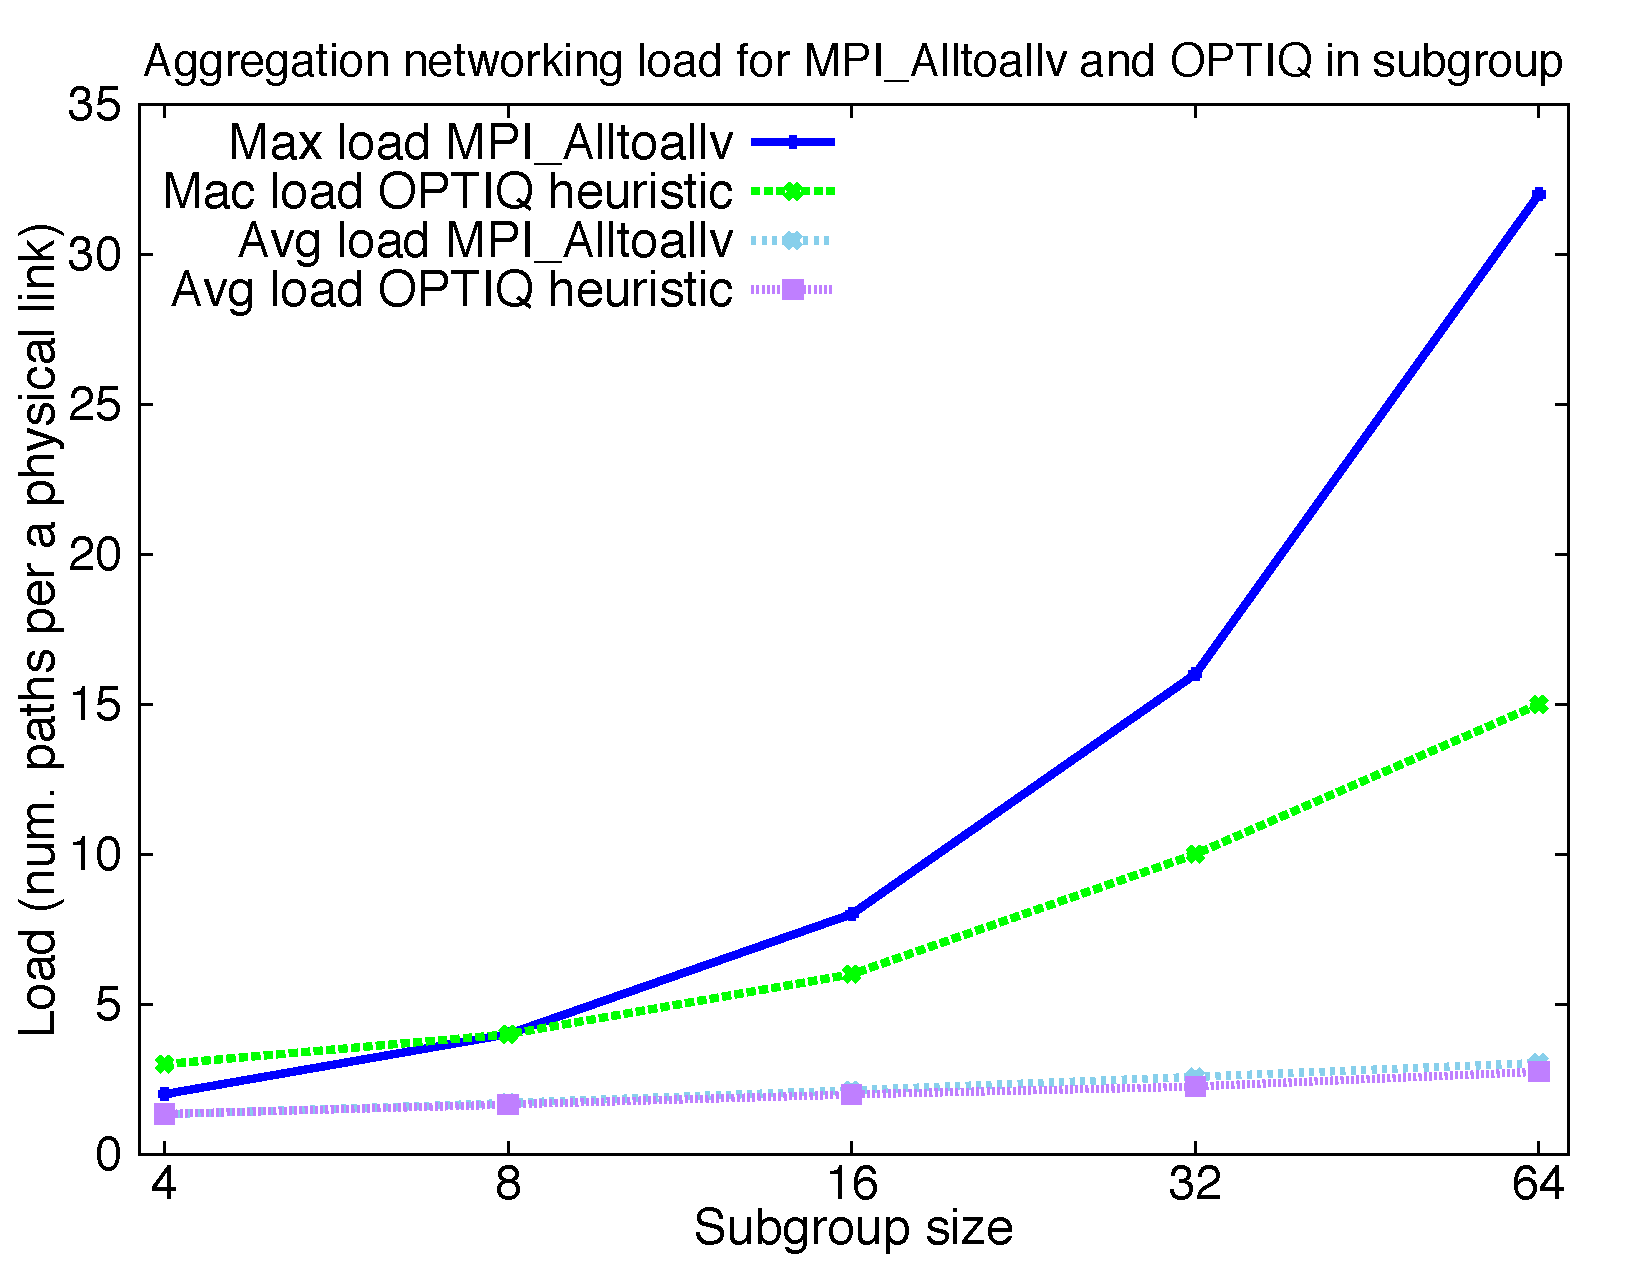
\includegraphics[scale=0.30]{figures/load.pdf}
\vspace{-0.1in}
\caption{Networking load over links}
\vspace{-0.1in}
\label{fig:aggload}
\end{figure}

Figure \ref{fig:aggload} shows the max and average loads for both MPI\_Alltoallv and OPTIQ. Load is number of paths that used a physical link. As we can see in the figure, when the group size increased the average load is approximate the same, but max load increased much faster in MPI\_Alltoallv compare to OPTiQ. This is because MPI\_Alltoallv used default routing algorithm. The default routing algorithm routes data in the longest dimension first leading to more load on certain links and no loads on many other links. Hence the max load in MPI\_Alltoalllv is higher than OPTIQ. Our work distributes the networking load over more links with lower max load. The networking distribution is shown in Figure \ref{fig:aggdist}

\begin{figure}[!htb]
\vspace{-0.1in}
\centering
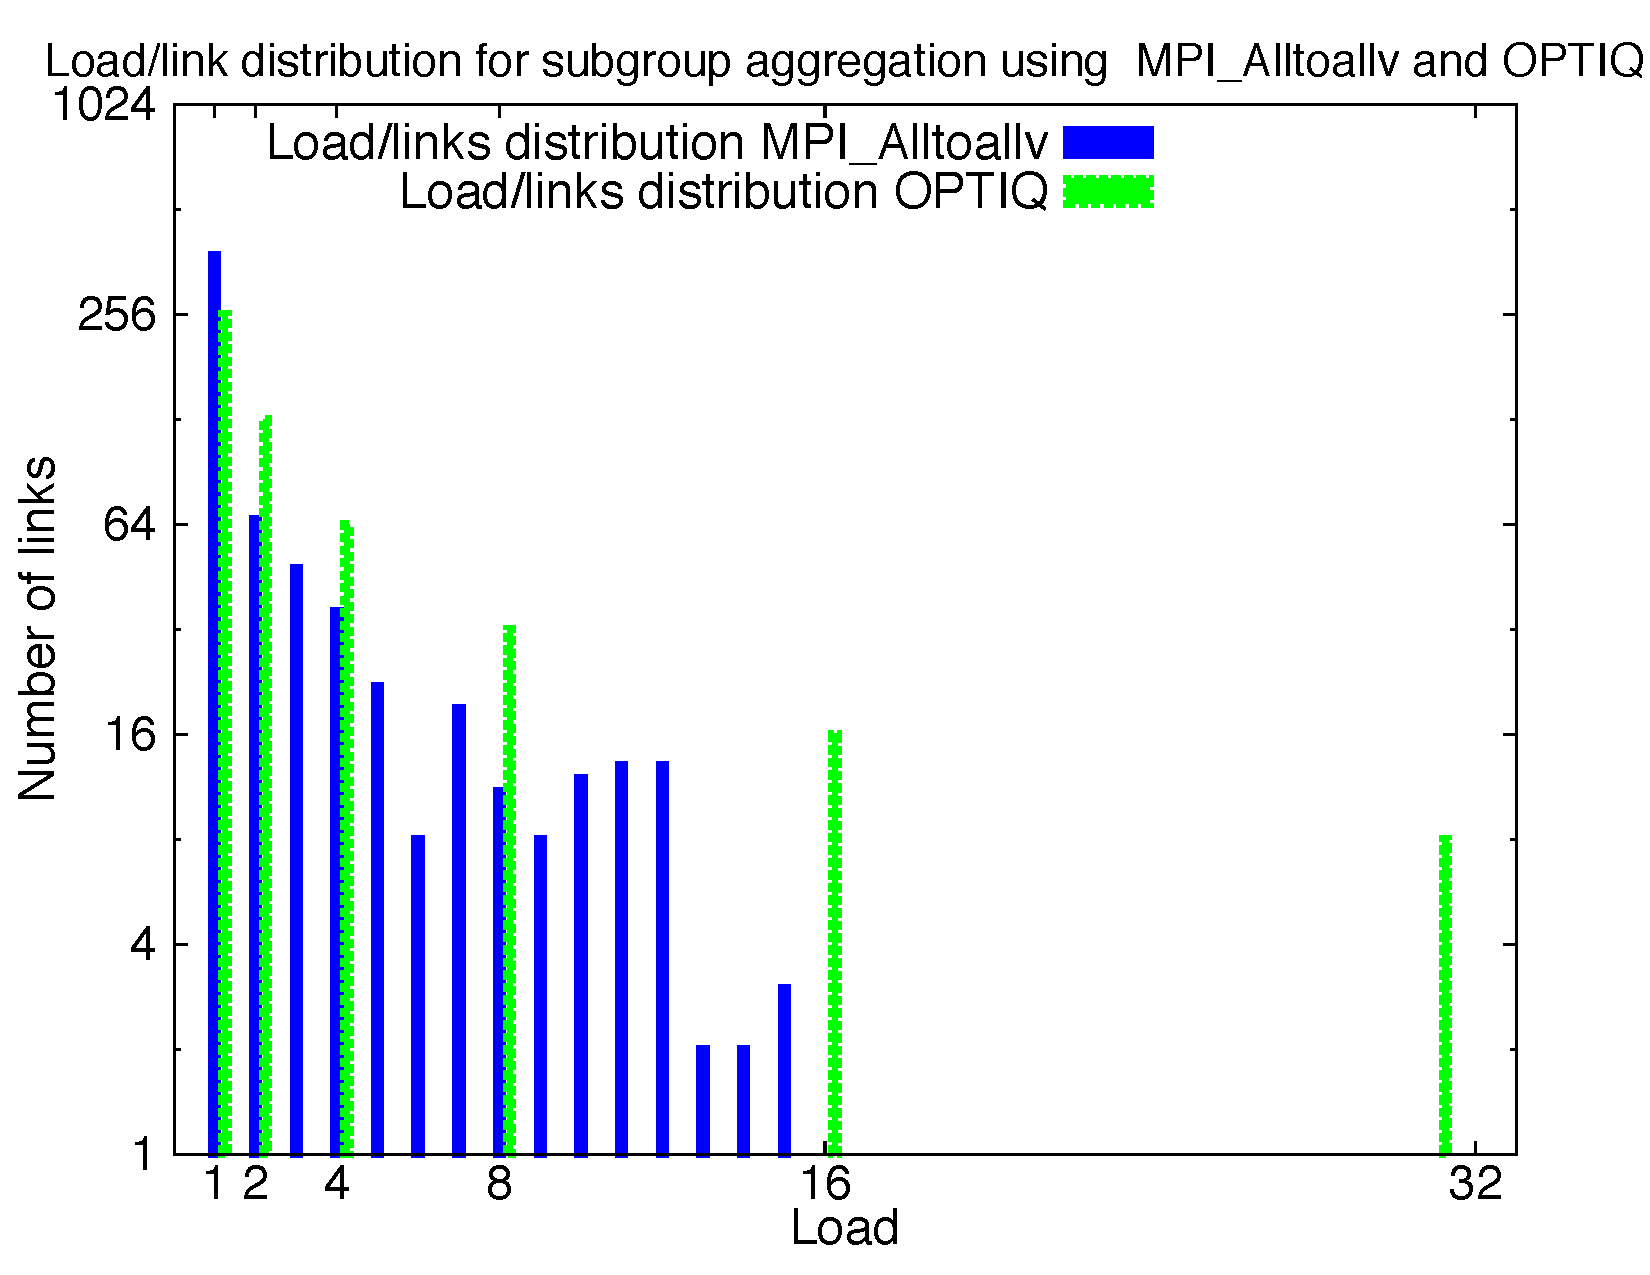
\includegraphics[scale=0.30]{figures/distribution.pdf}
\vspace{-0.1in}
\caption{Networking load disitribution over links}
\vspace{-0.1in}
\label{fig:aggdist}
\end{figure}

Figure \ref{fig:aggdist} shows that our work has a better networking load distribution. All of the loaded links have max load at most of 15, with many links has low load. While MPI\_Alltoallv has 8 links with max load of 32. We achieved better load distribution by using more links and by using longer links. This leads to a litte higher max hops (1 or 2 hops) and average hops used. The Figure \ref{fig:agghop} shows the maximum and average nuber of hops used.

\begin{figure}[!htb]
\vspace{-0.1in}
\centering
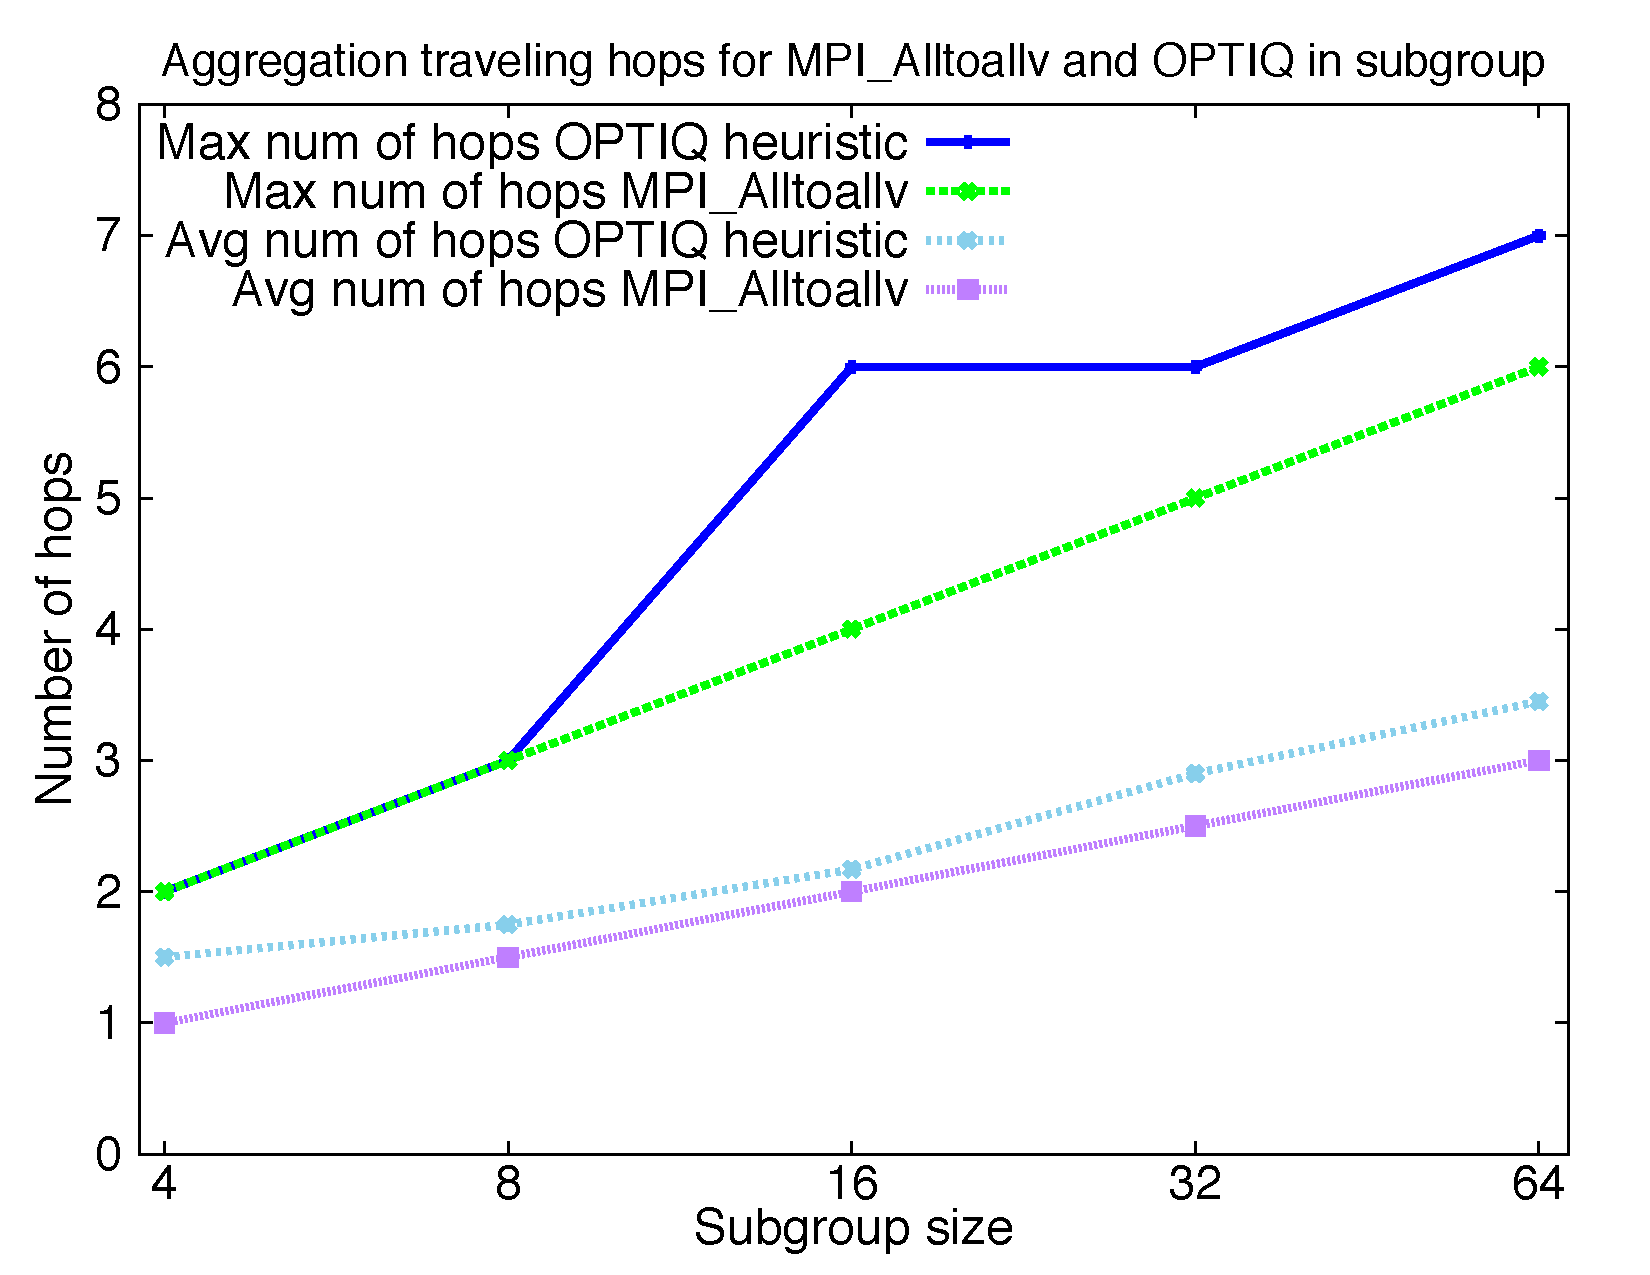
\includegraphics[scale=0.30]{figures/hop.pdf}
\vspace{-0.1in}
\caption{Max and average hops in data aggregation}
\vspace{-0.1in}
\label{fig:agghop}
\end{figure}

In the Figure \ref{fig:agghop} we can see that compare to MPI\_Alltoallv, OPTIQ used 1 to 2 hops more in case of maximum number of hops and 0.5 hops more in case of average number of hops. This is because OPTIQ explored longer paths to avoid increasing max load. The algorithms we have also try to balance between number of hops and max load as too long paths can actually increase time hence degrade data movement bandwidth.

\subsection{Scalability}
Show scalability by partition size, number of ranks per node and message sizes
